\section{ Katsekontakti }
\label{fs-hyppaamisen-perusteet-katsekontakti}


FS-hyppäämisen tärkein perusasia on katse. Katse on ainoa keino kommunikoida ilmassa. 


Katsetta käyttäen säilytetään myös kiintopiste hyppykaverissa tai muodostelman keskipisteessä. Yleisin syy tasoeroihin ja vaakaetäisyyden syntymiseen on katsekontaktin puuttuminen, koska vartalo pyrkii liikkumaan katseen suuntaan. 

\section{ Keskipiste }
\label{fs-hyppaamisen-perusteet-keskipiste}


Hyppääjän keskipiste sijaitsee navan kohdalla, mutta käännöksen keskipiste vaihtelee halutun käännöksen mukaan, esim. käännös polven ympäri. Myös jokaisella muodostelmalla on keskipiste, jonka suhteen muodostelmat rakennetaan. Esimerkiksi kahden hengen tähdessä keskipiste sijaitsee käsiotteiden keskellä. Sekvenssissä muodostelmat rakennetaan niin, että keskipiste pysyy jotakuinkin samassa kohtaa läpi sekvenssin. 

\section{ Otteiden ottaminen }
\label{fs-hyppaamisen-perusteet-otteiden-ottaminen}


Otteita otettaessa on hyppääjien oltava samalla tasolla. Otteet otetaan joko ranteista, käsi- tai jalkagripeistä. Otteen on oltava napakka, mutta siinä ei saa olla vetoa. Ote on muodostelman viimeistelyä tai kasaamista, eli hetkellinen pysähdys ennen muodostelman purkua, josta siirrytään seuraavaan muodostelmaan. Otteessa ei roikuta, vaan lennetään aktiivisesti omaa paikkaa ja ollaan valmiina siirtymään seuraavaan muodostelmaan. 

\section{ Box }
\label{fs-hyppaamisen-perusteet-box}


Vapaapudotuksen perusasento ja siinä liikkuminen löytyvät Laskuvarjohyppääjän oppaasta. (\ref{perusliikkeet-vapaassa-perusasento} s.\pageref{perusliikkeet-vapaassa-perusasento}) (\ref{fs-kuviohyppaaminen} s.\pageref{fs-kuviohyppaaminen}) 

\section{ Mantis }
\label{fs-hyppaamisen-perusteet-mantis}


Mantis on vapaapudotusasento, joka nykyisin on FS-hyppäämisen perusasento. Mantis mahdollistaa lyhyemmät, nopeammat ja aggressiivisemmat liikkeet kuin box. Erotuksena boxiin mantiksessa kädet ovat rinnan tasolla ja kyynärpäät alhaalla, polvet saavat roikkua. Asentoa muokkaa ilmavirta, eikä taivuttamista ja/tai lantion työntämistä alas tarvita. 


Mantiksen etuja boxiin verrattuna ovat lyhyemmät välimatkat hyppääjien välillä, parempi katsekontakti, helpompi otteiden ottaminen ja se, että pienetkin liikkeet ovat tehokkaita. Käsillä työskennellään boxiin verrattuna luonnollisemmassa asennossa, kun kädet ovat ylävartalon edessä. 


\begin{Figure}\centering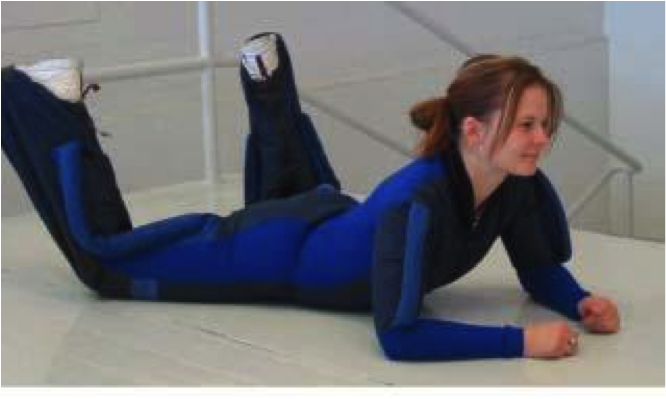
\includegraphics[width=0.95\textwidth]{Mantis.png}\captionof{figure}{Mantis-asento}\end{Figure} 

\subsection{ Mantiksen harjoittelu }
\label{fs-hyppaamisen-perusteet-mantiksen-harjoittelu}


Hyvä keino harjoitella mantista on esimerkiksi televisiota katsellessa maata lattialla kyynärvarret maassa, rintakehä ja pää kohotettuna (kuva) sekä jalat noin 90 asteen kulmassa, polvista taivutettuina. Tässä asennossa voi myös harjoitella käännöksiä, jotta käsien ja jalkojen yhtäaikainen liike jää lihasmuistiin. Erinomaisia mantis-harjoituksia ovat kaikki 2-way hypyt. Sidebody-hypyt ovat erityisen hyviä harjoituksia, koska oikea asento tulee luonnostaan, kun pyritään katsomaan toisen hyppääjän selän yli. 


\begin{Figure}\centering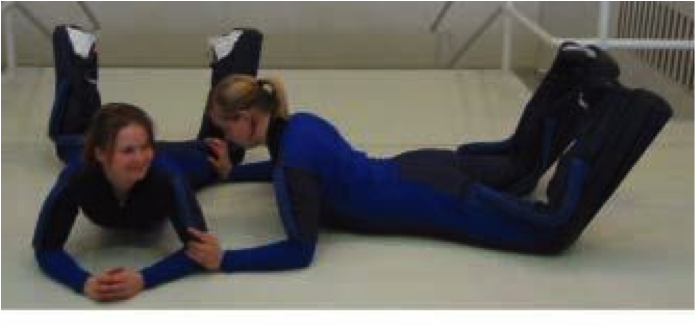
\includegraphics[width=0.95\textwidth]{Sidebody-harjoittelu.png}\captionof{figure}{Sidebody}\end{Figure} 

\section{ Turvallisuus }
\label{fs-hyppaamisen-perusteet-turvallisuus}


Joitakin turvallisuusasioita tarkistettavaksi ja huomioitavaksi: 


Ennen hyppyä: 

\begin{itemize}
\item  Mieti, onko sää sopiva omiin taitoihisi nähden.  
\item  Mieti, sopiiko hypyn vaativuus omiin taitoihisi.  
\item  Tarkista ja huolla omat varusteesi (huomioi aina luupin kunto ja tiukkuus).  
\item  Mieti, vaikuttavatko painot siipikuormaasi.  
\item  Pidä painovyötä haalareiden päällä ja varmista, että vyössä on pitävä, mutta helposti avattava lukitus (jos laskeudutkin veteen). 
\end{itemize}

Koneessa: 

\begin{itemize}
\item  Jos hyppykone on sinulle uusi, varmistu siitä, että tunnet sen hyppäämiseen vaikuttavat ominaisuudet (hätävarusteet ja hätäuloskäynnit, mahdollinen sakkausvaara, oven toiminta jne.)  
\item  Toimi sovittujen ohjeiden mukaan.  
\item  Tarkista omat varusteesi.  
\item  Tarkista hyppykaverisi varusteet.  
\item  Varmistu oikeasta uloshyppypaikasta.  
\item  Varmistu esteettömästä ja turvallisesta uloshypystä.  
\end{itemize}

Hypyllä: 

\begin{itemize}
\item  Varmista riittävä väli edelliseen ryhmään.  
\item  Etsi muut hyppääjät, jos uloshyppy hajoaa.  
\item  Varsinkin isoja kuvia hypätessäsi tarkkaile muita hyppääjiä vapaassa törmäyksen estämiseksi.  
\item  Tarkkaile korkeutta.  
\item  Liu'u riittävän pitkälle.  
\item  Varmista vapaa ilmatila.  
\item  Avaa oikeassa korkeudessa.  
\end{itemize}

Varjon varassa: 

\begin{itemize}
\item  Varaudu kuvun kääntymiseen avauksen jälkeen.  
\item  Tarkista varusteesi (\ref{hyppytapahtuma-varjon-avautuminen-ja-lentokuntoon-saattaminen} s.\pageref{hyppytapahtuma-varjon-avautuminen-ja-lentokuntoon-saattaminen}) 
\item  Tarkista, että hyppykaveriesi varjot ovat auki.  
\item  Tarkkaile ilmatilaa ja huomioi muut hyppääjät varjon varassa.  
\item  Jos et pääse maalialueelle, valitse ajoissa varalaskupaikka (tilanteen mukaan laskeudu samaan paikkaan kuin hyppykaverisi).  
\item  Noudata laskeutumiskuria ja sovittuja sääntöjä. 
\end{itemize}
